\documentclass[leqno,a4paper]{article}
\usepackage{hyperref}
\usepackage{caption}
\usepackage[T1]{fontenc}
\usepackage[utf8]{inputenc}
\usepackage{lmodern}
\usepackage[english]{babel}
\linespread{1.25} %easier reading/grading.
\usepackage{amsmath} %d'oh
\usepackage{amsfonts}
\usepackage{graphicx}
\usepackage{bold-extra} %for \mb
\usepackage[margin=2.5cm]{geometry} %for custom margins
\usepackage{enumerate} %for special counters
\usepackage{titlesec} %for section numbering
\usepackage{ifthen}
\renewcommand\thesubsection{\alph{subsection}}
\titleformat{\section}{\it \bf \large}{{\normalfont  \bf \thesection.}}{4pt}{}[]
\titleformat{\subsection}{\it \bf \large}{{\normalfont \bf \quad \large  \thesection \thesubsection)}}{5pt}{}[]
\titleformat{\subsubsection}{\bf \it}{\qquad}{5pt}{}[]

\numberwithin{equation}{section}
\newcommand\norm[1]{\left\lVert#1\right\rVert} %http://tex.stackexchange.com/questions/107186/how-to-write-norm-which-adjusts-its-size
\renewcommand{\O}{\mathcal{O}}
\renewcommand{\bf}{\bfseries}
\renewcommand{\sc}{\scshape}
\renewcommand{\it}{\itshape}
\renewcommand{\div}{\text{div }}
\renewcommand{\Re}{\mathbb{R}}
\newcommand{\op}{\left(}
\newcommand{\cp}{\right)}
\newcommand{\N}{\mathbb{N}}
\newcommand{\mb}{\mathbf}
\newcommand{\nn}{\\\nonumber}
\newcommand{\curl}{\text{curl }}
\newcommand{\inp}[2]{\left<#1, #2\right>}
\renewcommand{\d}[1]{\,\text{d}#1}
\newcommand{\pdrv}[2][x]{\frac{\partial #2}{\partial #1}}
\newcommand{\drv}[2][x]{\frac{\text{d} #2}{\text{d} #1}}
\renewcommand{\maketitle}[2][]{\begin{center}
{{\bf \huge \sc #2\\
\ifthenelse{\equal{#1}{}}{}{{\vspace{-12pt} \Large #1}\\\vspace{5pt}}
\large R.G.A. Deckers}}
\vspace{-1. cm}\rule[2.5 cm]{16 cm}{1 pt}
\vspace{-2.5 cm}
\end{center}}

\usepackage[]{algorithm2e}
\usepackage[T1]{fontenc}          % change font encoding to T1
\usepackage[framed,numbered]{matlab-prettifier}
\begin{document}
  \maketitle[Scientific Computing III]{Project 1}
\tableofcontents

\section{Creating the matrices \texorpdfstring{$K$}{\em K}, \texorpdfstring{$M$}{\em M}, and \texorpdfstring{$A$}{\em A}}
  First, before we can do anything else, we of course have to create our matrices.
  the function we use for doing so is given in listing \ref{ml:create_matrices}.
\section{Power method}
\subsection{Implementation}
The implementation of the power-method is given in listing \ref{ml:eig_power}.

\subsection{Convergence}
 Let $1 = |\lambda_1| \geq \ldots \geq |\lambda_n|$ be the eigenvalues of a matrix $A$ and $\vec e_1, \ldots, \vec e_n$ the corresponding eigenvectors.
 Then $A^k \vec x = \sum_{i=1} ^{i=n} a_i\lambda_i^k\vec e_i$. where $a_i$ are the eigenspace coefficients of $\vec x$.
 All eigenvectors with eigenvalues less than one converges to zero for $k\to\infty$, therefore if all $\lambda_i$ for $i\not = 1$ are smaller than $\lambda_1$ the rate of convergence in the first order
 will be $\left|\lambda_1/\lambda_2\right|$. If the dominant eigenvalue is not unique (down to a sign) than the eigenvalue will still convert, at a rate defined by the next eigenvalue less than $\lambda_1$ in the absolute, but the eigenvector will not.
\subsection{Results}
\subsubsection{Eigenvector}
The eigenvector is plotted in figure \ref{fig:eigenvectors}.
\subsubsection{Iterations vs. Matrix Size}
The iteration count is plotted in figure \ref{fig:iterations}.
\begin{figure}[h!]
  \centering 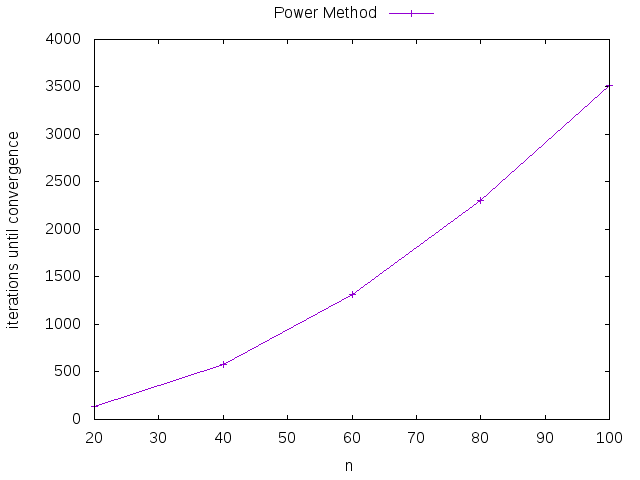
\includegraphics[width=0.75\textwidth]{plots/iterations_vs_n.png}
  \caption{Iterations required to find the largest and smallest eigenvalue of $A$}
  \label{fig:iterations}
\end{figure}
\subsubsection{Error}
The relative error is plotted in figure \ref{fig:error}.

\section{Inverse iteration}

\subsection{Implementation}
In order to implement inverse iteration,
we find the smallest eigenvector by
using power iteration over $A-\lambda_1 I$ and adding $\lambda_1$ to the result.
We then use power iteration over $(A-\lambda_n I)^{-1}$ to compute the corresponding eigenvector. We do however not compute the
inverse directly but use LU decomposition for faster iteration.
The technical implementation is shown in listing \ref{ml:inverse}.

\subsection{Convergence}
The inverse iteration converges linearly just like the power method. This is because, as described above, it can be implemented using
just power iteration.

\subsection{results}
\subsubsection{Eigenvectors}
The eigenvector is plotted in figure \ref{fig:eigenvectors}.
\begin{figure}[h!]
  \centering 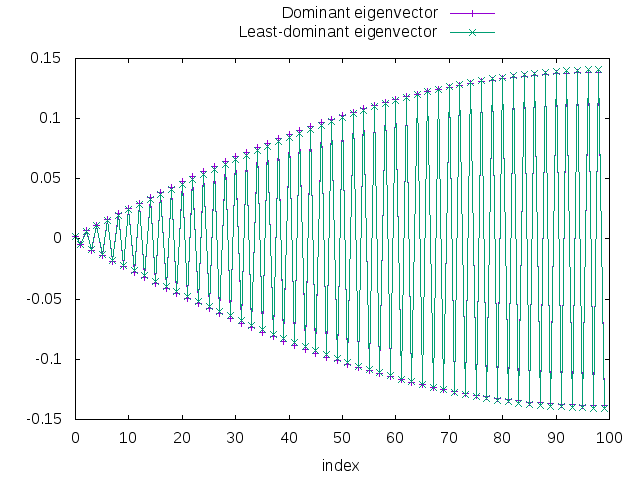
\includegraphics[width=0.75\textwidth]{plots/eigenvectors.png}
  \caption{eigenvectors corresponding to the largest and smalles eigenvalue.}
  \label{fig:eigenvectors}
\end{figure}

\subsubsection{iterations vs. matrix size}
The iteration count is plotted in figure \ref{fig:iterations_inverse}.
\begin{figure}[h!]
  \centering 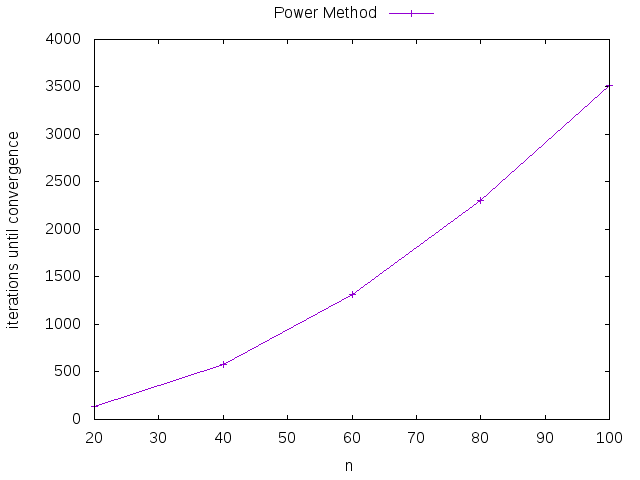
\includegraphics[width=0.75\textwidth]{plots/iterations_vs_n.png}
  \caption{Iterations required to find the largest eigenvector of $A$ using inverse iteration}
  \label{fig:iterations_inverse}
\end{figure}

\subsubsection{error vs. matrix size}
The relative error is plotted in figure \ref{fig:error}. The condition number a function of the matrix size is plotted in figure \ref{fig:cond}, this difference explains the difference in relative errors.
\begin{figure}[h!]
  \centering 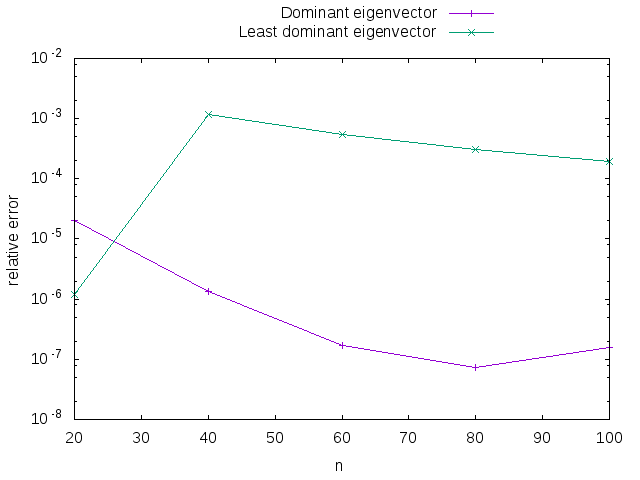
\includegraphics[width=0.75\textwidth]{plots/error_vs_n.png}
  \caption{Relative error of the power method corresponding to the largest and smalles eigenvalue as a function of matrix size.}
  \label{fig:error}
\end{figure}

\begin{figure}[h!]
  \centering 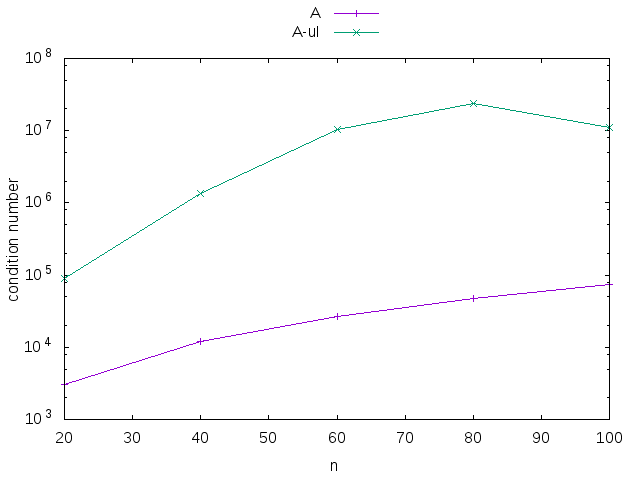
\includegraphics[width=0.75\textwidth]{plots/condition_number.png}
  \caption{Condition number of the A and B matrices as a function of matrix size.}
  \label{fig:cond}
\end{figure}

\newpage
\appendix
\section{Source Code} \label{appendix:source}

\lstinputlisting[
  label=ml:create_matrices,
  caption=Matlab function for creating our problem matrices.,
  style      = Matlab-editor,
  basicstyle = \mlttfamily,
]{matlab/create_matrices.m}

\lstinputlisting[
  label=ml:create_matrices,
  caption=Matlab function for creating our problem matrices.,
  style      = Matlab-editor,
  basicstyle = \mlttfamily,
]{matlab/inverse_iteration.m}

\lstinputlisting[
  label=ml:eig_power,
  caption=Matlab function for computing the dominant eigenvalue of a matrix using the power method.,
  style      = Matlab-editor,
  basicstyle = \mlttfamily,
]{matlab/eig_power.m}

\lstinputlisting[
  label=ml:part_01,
  caption=Matlab script used to generate the data.,
  style      = Matlab-editor,
  basicstyle = \mlttfamily,
]{matlab/part_01.m}

\end{document}
